\section{创建 AHAPE 抽象类}
\hfill\ctli{实验时间}{~2015~年~1~月~14~日}
\subsection*{【实验目的】}
\begin{enumerate}[topsep=0pt,partopsep=0pt,itemsep=0pt,parsep=0pt,label={\arabic*、}]
\item 掌握多态性的概念。
\item 掌握虚函数概念及其与多态性的关系。
\end{enumerate}
\subsection*{【实验环境】}
\MyEnvironment
\subsection*{【实验内容】}
%功能要求:
定义一个抽象类SHAPE,抽象方法SHAPE包含X和Y两个属性的访问方法,VOLUME 方法,AREA抽象方法和GETNAME方法。不同的形状类,如POINT 类实现SHAPE 类,RECTANGLE类继承PIONT ,ELLIPSE 类继承RECTANGLE 类。CIRCLE 类继承ELLIPSE 类,CYLINDER类继承CIRCLE类。创建每个类的实例,并将每个类的实例存放于类型为SHAPE的数组中。以该SHAPE的数组作为参数,调用参数的类型为SHAPE 的数组的SHOWSHAPINFO方法,通过调用重写的方法为相应得图形对象计算表面积,体积并输出图形的名称。
\subsection*{【详细分析】}
图~\ref{exp07classes}~展示了各个类之间的关系。

\newcommand\method[2]{{#1}:~{\it #2}}
\newcommand\vart[2]{{#1}:~{\it #2}}
\newcommand\argu[2]{{\sf #2}:~{\it #1}}
\newcommand\comt[1]{\hfill\quad{\tt //#1}}
\newcommand\comtn[1]{\\\comt{#1}}

\begin{figure}[htp]
\linespread{1}\centering\small
\begin{tikzpicture}[scale=1.2]
\umlclass[type=abstract,x=0,y=1]{SHAPE}{
-- \argu{double}{x}\\
-- \argu{double}{y}\\
}{
+ \method{VOLUME()}{double} \{abstract\}\\
+ \method{AREA()}{double} \{abstract\}\\
+ \method{GETNAME()}{std::string} \{abstract\}\\
+ \method{SHOWSHAPINFO()}{void} \{abstract\}\\
}
\umlemptyclass[x=0, y=-2]{POINT}
\umluniassoc[geometry=--]{POINT}{SHAPE}
\umlemptyclass[x=0, y=-4]{RECTANGLE}
\umlinherit[geometry=--]{RECTANGLE}{POINT}
\umlemptyclass[x=0, y=-6]{ELLIPSE}
\umlinherit[geometry=--]{ELLIPSE}{RECTANGLE}
\umlemptyclass[x=0, y=-8]{CIRCLE}
\umlinherit[geometry=--]{CIRCLE}{ELLIPSE}
\umlemptyclass[x=0, y=-10]{CYLINDER}
\umlinherit[geometry=--]{CYLINDER}{CIRCLE}
\end{tikzpicture}
\par\vspace*{1cm}\par
\caption{\label{exp07classes}AHAPE 抽象类}
\end{figure}

\subsection*{【实验源码】}
{\linespread{1}\lstinputlisting[caption={\tt AHAPE.cpp}]{exp07/ASHAPE.cpp}}
\subsection*{【实验结果】}
\begin{figure}[htp]
\centering
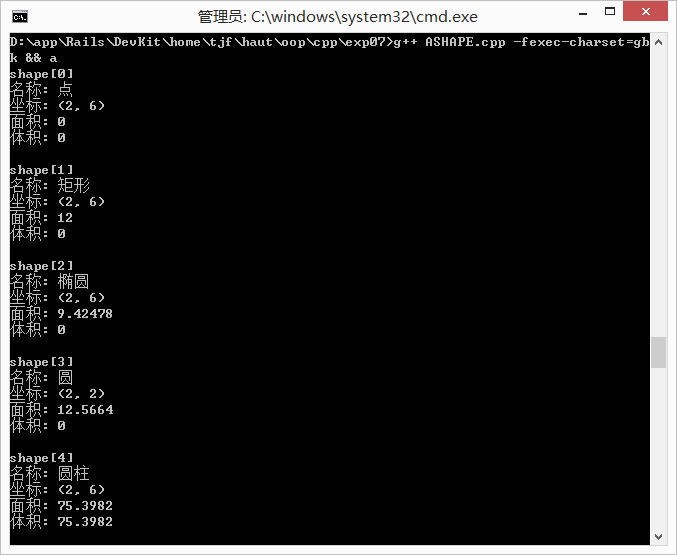
\includegraphics[width=\textwidth]{exp07/ASHAPE.png}
\caption{\label{out07_01}AHAPE 抽象类}
\end{figure}
\subsection*{【实验体会】}
这个题目是比较典型的多态练习题,虽然在逻辑上这几个继承真心说不过去,但是题目终究是题目,和现实区别还是“不要在意这些细节”。而且这个全大写的命名方式还是让我恶心了半天,是回到了60年代了吗?

题目本身并不难,画出来继承关系图就清楚许多了。抽象类的方法设置成 virtual = 0,然后它的子类一个个按照题目叙述继承,并实现各自的方法。由于它们有一个共同的抽象父类,所以可以存在相同类型的数组中,这大大方便了操作。这个题目对于巩固抽象类 \{abstract\} 概念很有帮助。
